\chapter{Grundlagen} \label{cha:Grundlagen}

\section{Java Virtual Machine} \label{sec:JVM}

  % java einleitung
  Gemessen am Interesse der Anwender und an ihrer Verbreitung ist Java die erfolgreichste Programmiersprache der letzten Jahre. Der Erfolg kam mit der Objektorientierung sowie der Plattformunabhängigkeit. Diese Fähigkeiten brachten eine große und fähige Kommune zusammen, die sowohl aus der Wirtschaft als auch aus dem Forschungsbereich stammt. Dementsprechend ist Java im Laufe der Zeit durch Designmuster, Architekturkonzepte, Paradigmen und aktuellen Sicherheit- sowie Industriestandrats erweitert worden. Da \textsc{Renew} mithilfe der Java Plattform umgesetzt wurde, kann sie sie sich alle gegebenen Vorteile zunutze machen. \newline
  Einer der wichtigen Bausteine von Java, ist die virtuelle Maschine, die das Suchen, Laden und Ausführen einer Codebasis auf allen gängigen Betriebssystemen erlaubt. Demzufolge spielt das Laden von Klassen aus örtlich unabhängigen Komponenten eine große Rolle für die entstandene \textsc{Renew} Architektur, denn die Plugins müssen gefunden, geladen und kommunikationsfähig eingerichtet werden, sodass sie sich gegenseitig nutzen und beeinflussen können.\bigbreak

  % Kapitelübersicht
  In diesem Kapitel werden grundlegende Konzepte des \textit{ Klassenpfads, Classloaders} und \textit{Reflection} erläutert, mithilfe dessen die \textsc{Renew} Plugin-Architektur umgesetzt wurde.


\section{Klassenpfads} \label{sec:K}

  % Klassenpfad Einleitung
  Jede Java-Anwendung wird zuerst in einer für Menschlich verständlichen Sprache geschrieben und anschließend in Byte-Code übersetzt. Infolgedessen ist der Code einsatzbereit für die Ausführung und wird an die virtuelle Maschine weiter gereicht.

  % Aufgabe des Klassenpfads 
  Um die kompilierten Klassen zu laden, wird von der virtuellen Maschine Ortsangaben mit entsprechendem Code erwartet. Die Ortsangaben nennt man \textit{Classapth} oder Klassenpfad. Dieser beschreibt eine Liste von Orten, an denen sich die zur Ausführung benötigten Klassen befinden, wie zum Beispiel das lokalen Dateisystem, das Netzwerk oder sogar die Datenbank. 

  % Ergebniss des Klassenpfad
  Nachdem der Klassenpfad für die entsprechenden Klassenlader gesetzt ist, kann das \textit{Classlaoder System} die gewünschten Klassen erfassen und in die virtuelle Maschine laden.

  \begin{figure}[h]
    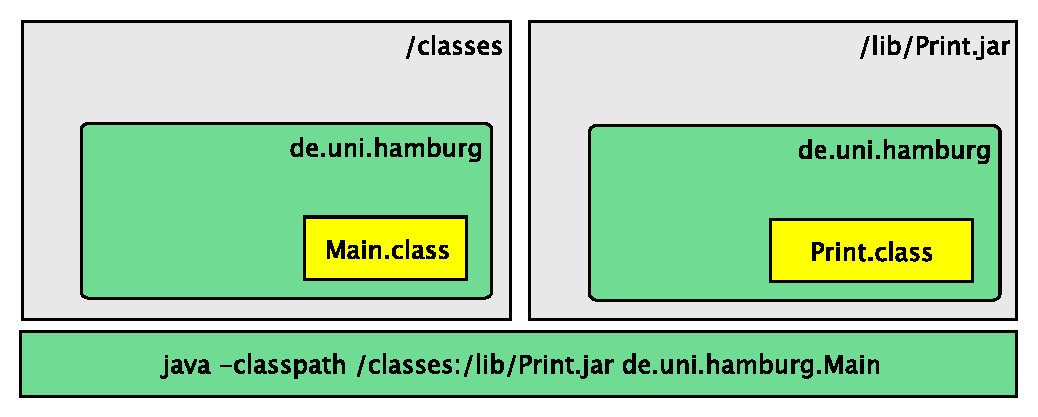
\includegraphics[width=\textwidth]{material/images/Classpath2.pdf}
    \caption{Java Classpath}
    \label{fig:cps}
  \end{figure}

  % Klassenpfad Zusammensetzbar  
  Im Beispiel \ref{fig:cps} besteht der Klassenpfad aus einem Verzeichnis sowie einem JAR Archive, die für die Ausführung nötige Klassen umfassen. Da beide Orte eine Dateistruktur beinhalten, unterliegen sie einer Einschränkung: beide müssen die Paketstruktur der Java Klassen widerspiegeln, so dass der \textit{Applikation Classloader} diese durchsuchen kann. Abschließend braucht Java einen Startpunkt, mit dem die Applikation ihre Ausführung beginnt. 

  % Classloading mit Richtung 
  Beim Starten der Applikation werden Klassen instanziiert, indem der Klassenpfad, von links nach rechts, nach dem benötigten Typ durchsucht und diese erstellt. Somit hat der Klassenpfad eine interne Ordnung und eine Abarbeitungsreihenfolge. 

  \begin{figure}[h]
    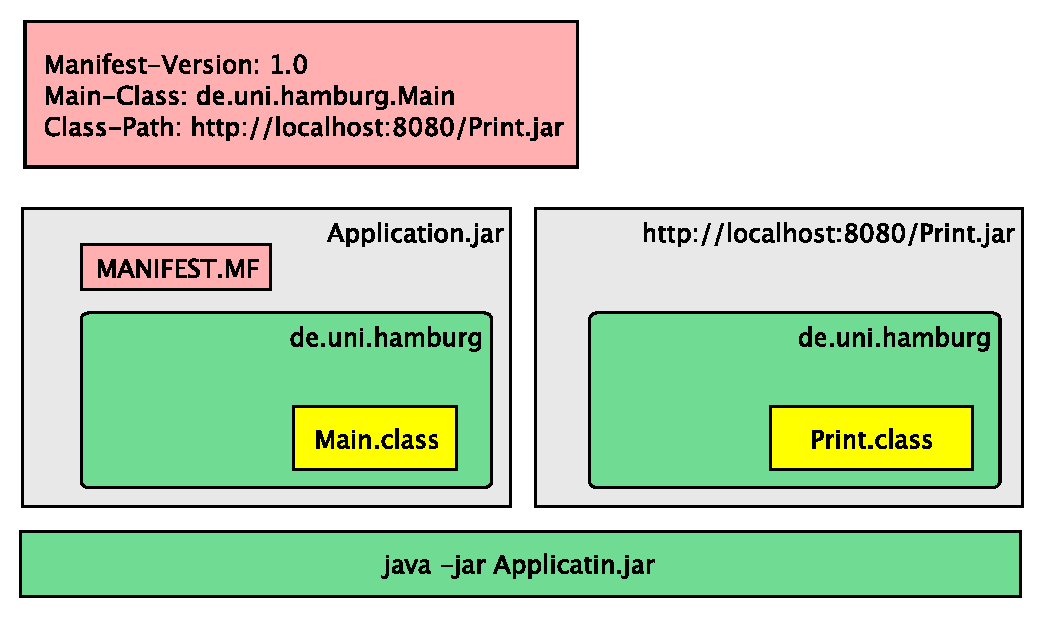
\includegraphics[width=\textwidth]{material/images/Classpath-Manifest2.pdf}
    \caption{Jar Classpath}
    \label{fig:cpa}
  \end{figure}

  % Erweitere Klassenpfad mit dem Manifest 
  Im Beispiel \ref{fig:cps} wurde explizit ein Applikationsklassenpfad gesetzt, der für die Ausführung benötigten Klassen zuständig ist. Für den Ablauf großer Applikationen mit viele Abhängigkeiten kann dieser ausgedehnt und chaotisch werden. Von daher bietet Java eine Archivstruktur, die einen standardisierten Aufbau sowie zusätzliche Meta-Information über den Container in sich trägt. 
  
  % Manifest Meta-information 
  Dank der Java Strukturrichtlinie, befindet sich der komplette Inhalt eines Archivs auf dem Applikationsklassenpfad und kann zusätzlich in der \textit{manifest.mf} Datei erweitert werden. Die \textit{manifest.mf} spielt eine große Rolle in der Entwicklung von Java Applikation, diese kann den Namen, die Version, den Entwickler und die Sicherheitsattribute tragen, die während der Laufzeit ausgewertet werden können. Zum Beispiel wird in \ref{fig:cpa} der Klassenpfad durch ein Archiv aus dem Web erweitert und für die Ausführung genutzt. Des Weiteren hält die \textit{manifest.mf} einen Einstiegspunkt für die Ausführung, der auf eine Klasse mit der \textit{main} Methode verweist.\newline
  Somit kann die Applikation in einer kurzen und einfachen Form gestartet werden, da der Ausführungskontext durch die Struktur und die mitgelieferte Meta-Information komplett ist. \cite{classLoadingOracle}


\section{Classloader}\label{sec:cl}

  % Aufteilung der Verantwortung 
  In den vorherigen Beispielen [\ref{fig:cps}, \ref{fig:cpa}] wurde die Bedeutung und die Rolle des Klassenpfads für die Applikation beschrieben, dennoch muss dieser zuerst verarbeitet werden. Diese Aufgabe wird von dem Classloader übernommen, der eine zentrale Rolle in jeder Applikation spielt, weil er nach benötigten Java Klassen für die Instantiierung der entsprechenden Typen sucht. Da es eine wichtige Aufgabe ist, wird die Verantwortung für das Laden der Klassen über eine Menge von Classloader aus dem \textit{Classloader System} aufgeteilt. 


  \subsection{Classloader System} \label{sec:cls}

    % Gründe 
    Das \textit{Classloader System} besteht aus drei integrierten Classloadern, von denen jeder einen anderen Gültigkeitsbereich für das Laden der Klassen besitzt. Beim Abstieg der Hierarchie wird der Umfang der verfügbaren Quellen breiter und weniger vertrauenswürdig. 

    \begin{figure}[h!]
      \centering
      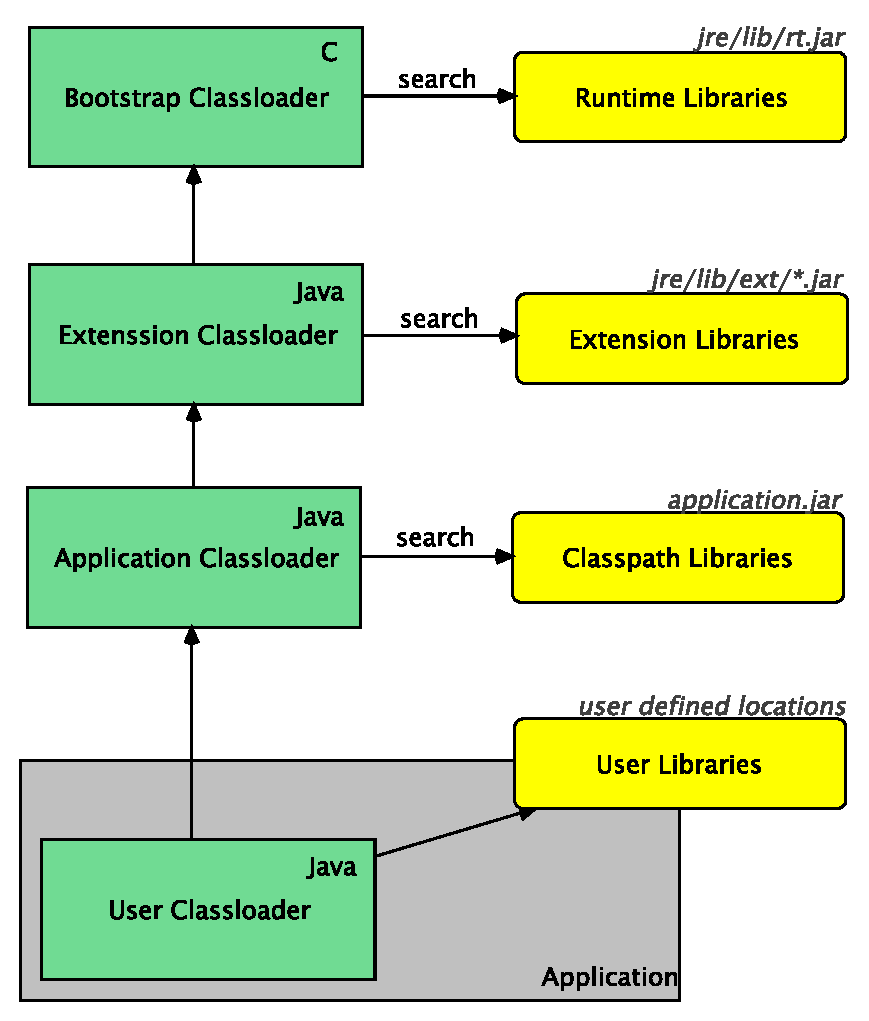
\includegraphics[width=0.7\textwidth]{material/images/Classloader-Hierarhie2.pdf}
      \caption{Classloader System \cite{classLoadingIntro}}
      \label{fig:cl}
    \end{figure}
    
    % Aufbau
    Oben in der Hierarchie befindet sich der \textit{Bootstrap-Classloader}. Dieser Classloader ist verantwortlich für das Laden der grundlegenden Java Klassenbibliothek, wie zum Beispiel Java-Core-API aus der \textit{rt.jar}. Diese Klassen sind am vertrauenswürdigsten und werden zum Starten der virtuellen Maschine verwendet. Der Classloader für Erweiterungen kann Klassen  aus dem Standarderweiterungspaket im Erweiterungsverzeichnis \textit{lib/ext} dazu laden. Diese können Java-UI wie kryptografische Erweiterungen beinhalten. Der darunter liegende \textit{Applikation Classloader} ist zuständig für unseren Code und lädt Klassen aus dem allgemeinen Klassenpfad einschließlich der zu startenden Anwendung. Zuletzt können benutzerdefinierte Classloader erstellt werden, die sich auf der unteren Ebene der Classloader-Hierarchie befinden und auf Drittanbieter Bibliotheken zugreifen können. Demzufolge sind diese Quellen nicht sicher genug, um eine große Priorität zuzuweisen, wie zum Beispiel den geladenen Klassen des \textit{Bootstrap-Classloader}.\bigbreak 
    % Delegierungsmodell übergang
    Das in \ref{fig:cl} abgebildete Classloader System verhindert, dass der Code aus weniger sicheren Quellen vertrauenswürdige Core-API-Klassen ersetzt, indem derselbe Name als Teil der Core-API angenommen wird. Daraus folgt ein Delegierungsmodell, welches eindeutige Klassen garantiert, da die Klassensuche von Oben nach Unten der Classloader-Hierarchie abgearbeitet wird.  \cite{classLoadingIntro} 
    

  \subsection{Delegierungsmodell} \label{sec:dm}
    
    % Suchalgorithmus  
    Das \textit{Classloader System} delegiert jede Anfrage zum Laden einer bestimmten Klasse zuerst an seinen übergeordneten Classloader, bevor der angeforderte Classloader versucht die Klasse selbst zu laden. Jeder Classloader hält somit einen Verweis auf einen übergeordneten Classloader und ist Teil eines Classloader Baums mit dem \textit{Bootstrap-Classloader} an der Wurzel. 

    % Rekursiv 
    Wenn eine Instanz einer bestimmten Klasse benötigt wird, prüft der Classloader, der die Anfrage bearbeitet, normalerweise mit seinem übergeordneten Classloader vorab. Der übergeordnete Classloader durchläuft wiederum den gleichen Prozess bis die Delegierungskette den \textit{Bootstrap-Classloader} erreicht. Sobald der \textit{Bootstrap-Classloader} erreicht wurde, beginnt die tatsächliche Suche nach der gewünschten Klasse.

    \begin{figure}[h]
      \centering
      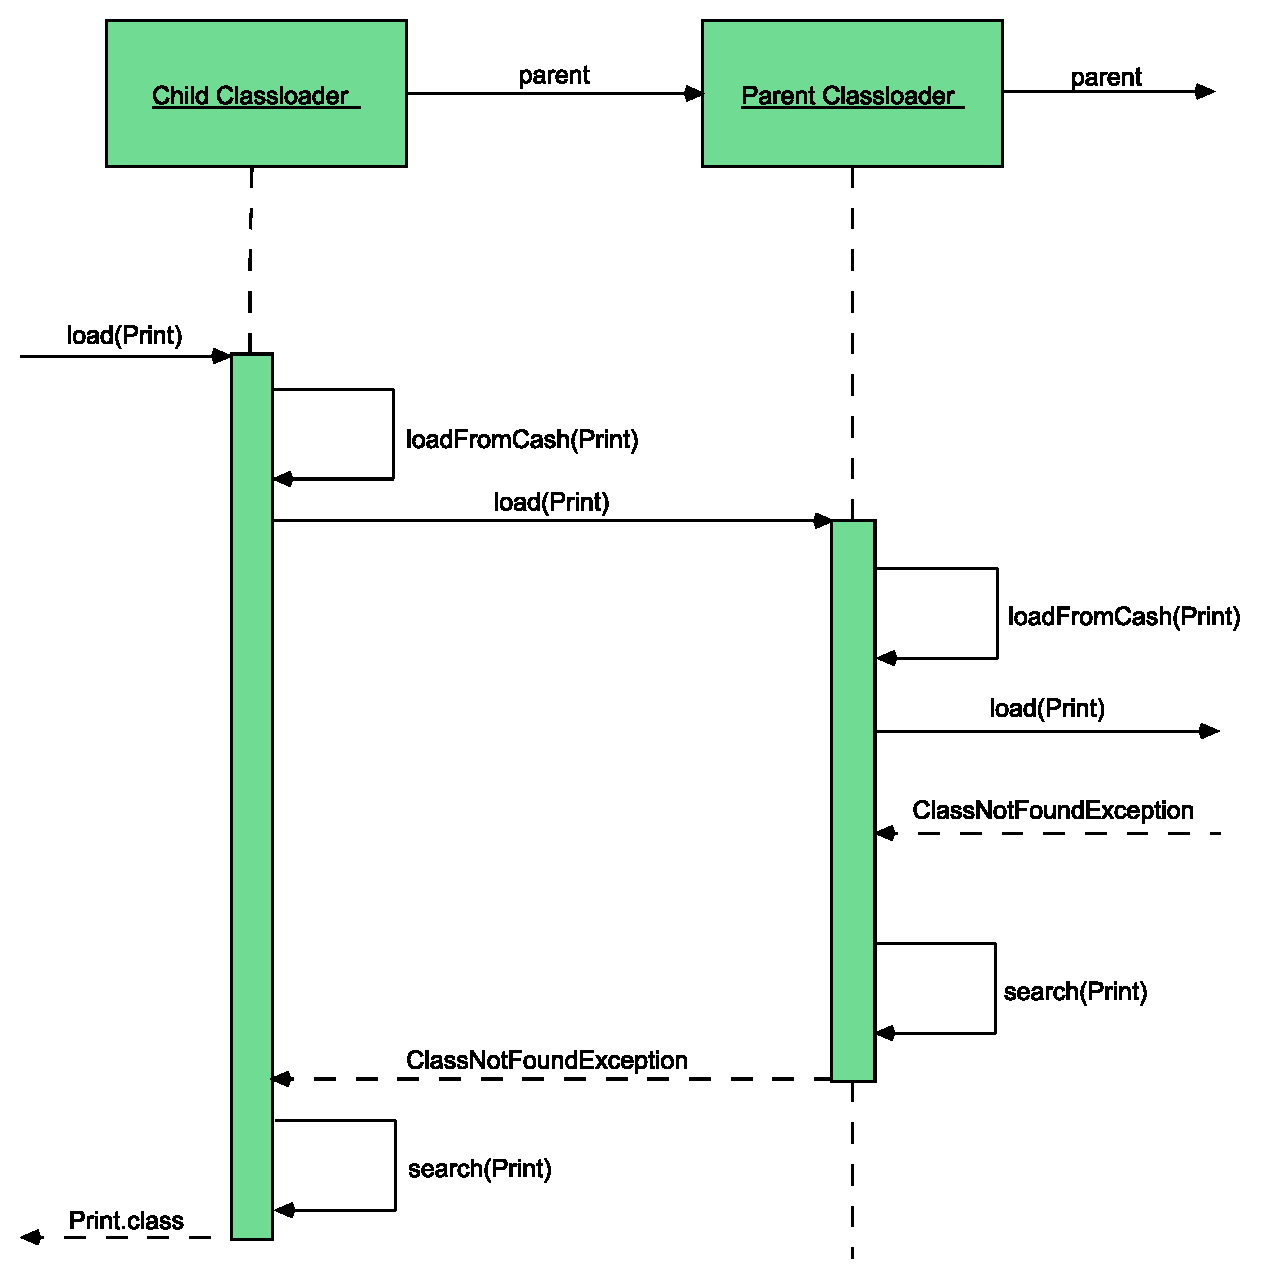
\includegraphics[width=0.9\textwidth]{material/images/flussCL.pdf}
      \caption{Klassensuche \cite{Forman04javareflection}}
      \label{fig:deligation}
    \end{figure}

    % Sichtbarkeit und Hierarchie 
    Wenn während der Suche ein übergeordneter Knoten eine bestimmte Klasse findet, dann wird diese Klasse die Baumhierarchie herunter zu der Anfrage delegiert. Andernfalls versucht der zuständige Classloader als letzter die Klasse selbstständig zu laden. Dies bedeutet, dass eine Klasse normalerweise nicht nur in dem Classloader sichtbar ist, der sie geladen hat, sondern auch für alle untergeordneten Instanzen. Dies bedeutet auch, wenn eine Klasse von mehr als einem Classloader in einem Baum geladen werden kann, wird immer die Klasse des übergeordneten Classloader eingelesen priorisiert. Dennoch wird vor jedem Laden der Klasse der Cash-Speicher des Classloaders nach der gewünschten Instanz durchsucht. Wenn diese existiert, wurde die Suche bereits zuvor durchgeführt und keiner der übergeordneten Classloader außer dem jetzigen war fähig die Anfrage zu beantworten. Somit kann die Suche beschleunigt werden, indem der Typ sofort zurückgegeben wird. \cite{parentDelegationModel}


  \subsection{Namensräume} \label{sec:nam}

    Geladene Klassen werden sowohl durch den Klassennamen als auch durch den Classloader eindeutig identifiziert. Demzufolge werden geladene Klassen in \textit{Namensräume} unterteilt, die vom \textit{Classloader System} individuell behandelt werden \cite{namespaces}. 

    % Idee 
    Ein \textit{Namensraum} ist eine Gruppe von Klassennamen, die von einem bestimmten Classloader geladen worden sind. Wenn ein Eintrag für eine Klasse einem \textit{Namensraum} hinzugefügt wurde, ist es nicht möglich, eine andere Klasse mit demselben Namen und unterschiedlichen Inhalt in den gleichen \textit{Namensraum} einzubinden. Nichtsdestotrotz können mehrere Kopien einer beliebigen Klasse in die Applikation geladen werden, indem für jede Klasse ein Classloader mit dem separaten \textit{Namensraum} erstellt wird \cite{customClDiffSpace}. 

    \begin{figure}[h]
      \centering
      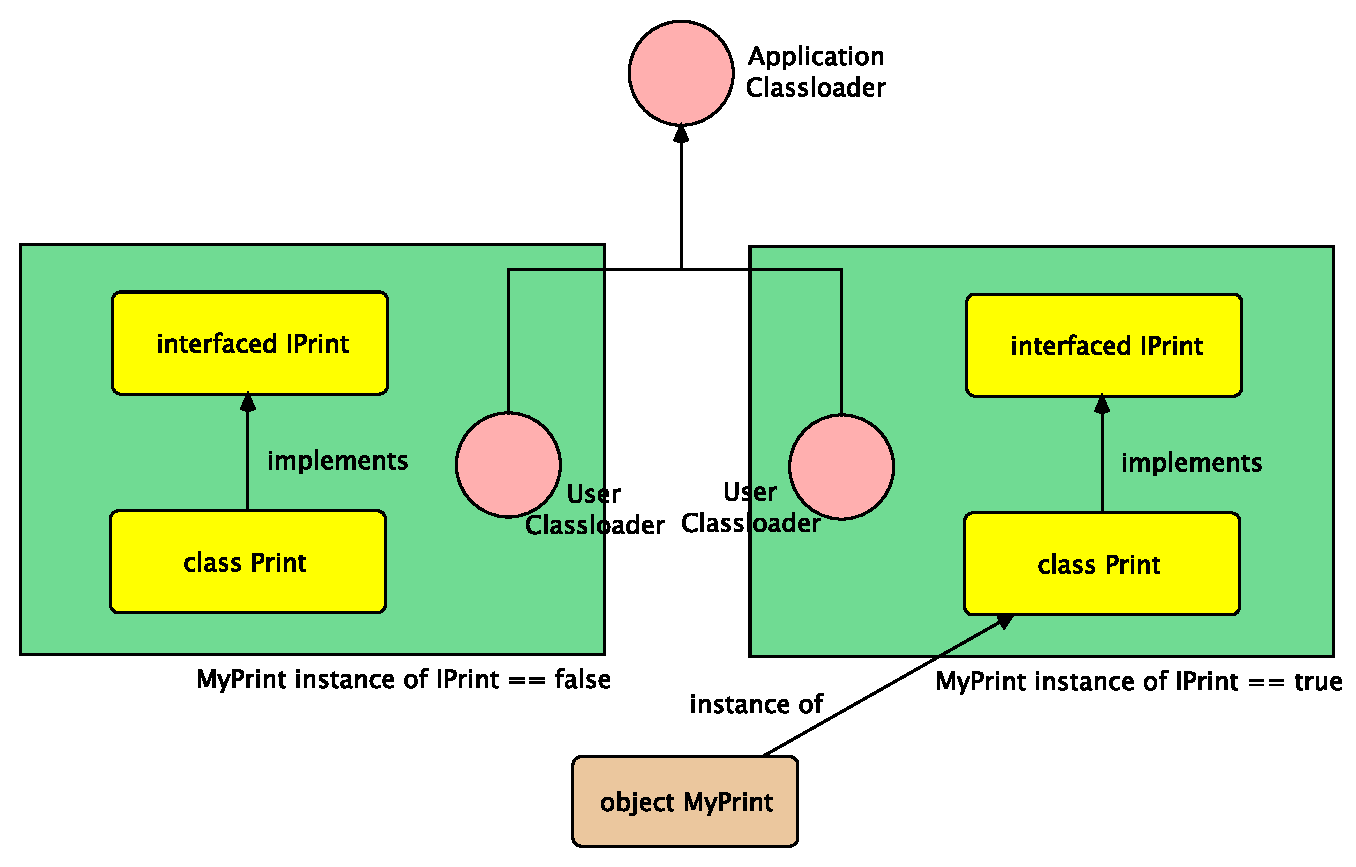
\includegraphics[width=0.9\textwidth]{material/images/namespace.pdf}
      \caption{Namensräume \cite{customClDiffSpace}}
      \label{fig:nam}
    \end{figure}

    % Ungleichheit identischer Klassen 
    Die Abbildung \ref{fig:nam} zeigt ein Beispiel für eine Klassenidentitätskrise, die sich ergibt, wenn eine Schnittstelle und die zugehörige Implementierung jeweils von zwei separaten Classloader geladen werden. Obwohl die Namen und binären Implementierungen der Schnittstellen und Klassen gleich sind, kann eine Instanz der Klasse von einem Classloader nicht als Implementierung des Interfaces von dem anderen Classloader erkannt werden. Bei Wunsch kann dieser Umstand gelöst werden, indem das Interface eine Ebene höher rutscht und von den Applikation Classloader geladen wird. Somit implementieren beide \textit{Print} Klassen dieselbe Schnittstelle.\bigbreak 

    % Schutz des Codes 
    Der Klassen Namensraum bietet zusätzliche Sicherheitsfunktionen wie die Kapselung privat deklarierter Pakete. Denn die Namensräume verhindern, dass der weniger vertrauenswürdige Code, der aus der Applikation oder benutzerdefinierte Classloader geladen worden ist, direkt mit mehr vertrauenswürdigen Klassen interagieren kann. Beispielsweise wird die Kern-API vom \textit{Bootstrap-Classloader} geladen, diese kann \textit{package private} Code enthalten, der bei Anfrage nicht an die unterliegende Classloader weitergereicht wird.


    % Schutz der privaten Pakete 
    Auch wenn ein untergeordneter Classloader die Paketstruktur der Core-API nachahmt, wird diese nicht als Teil der Java Core-API anerkannt, da dieser von den falschen Classloader geladen wurde. Somit verhindert die Verwendung von Namensräumen die Möglichkeit spezielle Zugriffsberechtigungen auf private Pakete zu erhalten, indem man selbst geschriebenen Code diesen zuweist. \cite{Forman04javareflection}


\section{Schnittstellen} \label{sec:kap}
  
  % Funktion 
  Die Schnittstelle und dessen Implementierung spielt eine entscheide Rolle für das Nutzen der Klassenfähigkeit. Eine Schnittstelle ist ein Vertrag, die die Funktionalität aller Klassen, die dieses implementieren beschreibt. Wenn eine Klasse eine bestimmte Schnittstelle implementiert, verspricht sie die Umsetzung aller in der Schnittstelle deklarierten Methoden.

  \begin{figure}[h!]
    \centering
    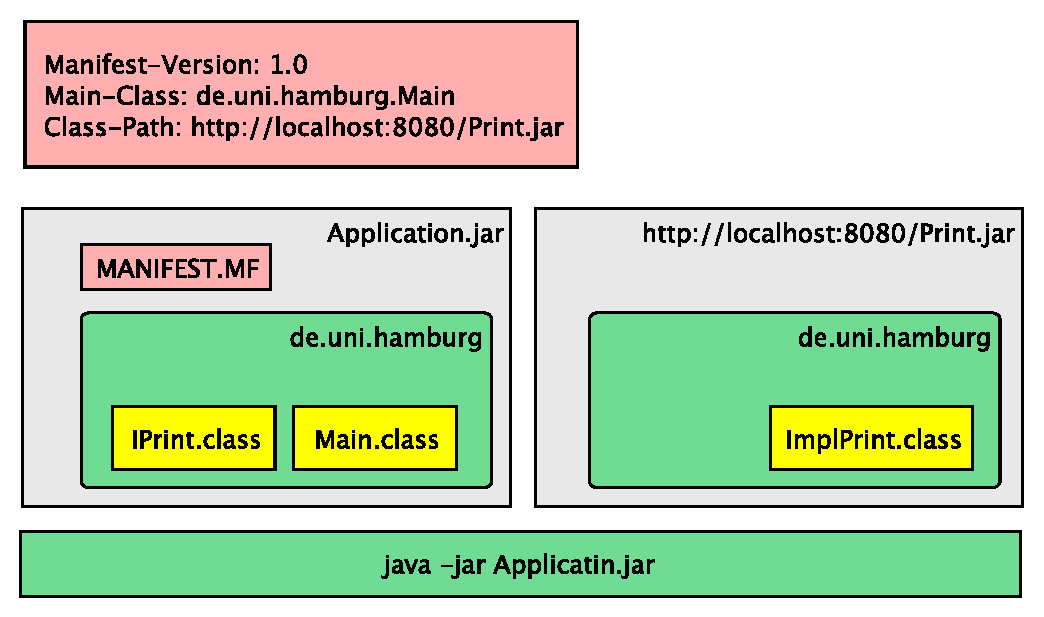
\includegraphics[width=0.8\textwidth]{material/images/Classpath-Interface-Implimentation.pdf}
    \caption{Schnittstelle}
    \label{fig:schnitt}
  \end{figure}

  % ist ein Garantie
  Somit wird durch die eigene Umsetzung des Schnittstellenvertrags ein mögliches Verhalten für die Nutzer der Schnittstellenbeschreibung implementiert. Daraus folgt ein Kommunikationsvertrag zwischen zwei Objekten, denn wenn eine Klasse eine Schnittstelle implementiert, implementiert diese alle in dieser Schnittstelle deklarierten Methoden und der Methodenaufruf an dieser Klasse wird garantiert ausgeführt.\cite{bloch2017effective}\bigbreak 
  
  % Dynamische Klassenbindung 
  Im Beispiel \ref{fig:schnitt} wird der Vorteil des Schnittstellenvertrags demonstriert, der das Ausführen der unbekannten \textit{PrintImpl} Umsetzung, durch eine einfache Schnittstellenbeschreibung \textit{IPrint} garantiert. Solange die Implementation sich auf derselben Klassenpfadhierarchie befindet wie die Schnittstelle, wird diese während der Laufzeit auf Kompatibilität geprüft und angewandt. Somit können dynamische Klassenbindungen während der Laufzeit entstehen und Laufzeitbibliotheken ausgetauscht werden, ohne dass die Applikation verändert wird. Hätte man die Schnittstelle nicht genutzt, würde man die Implementation nur als ein Objekt Type instanziieren können und hätte keinen einfachen Zugriff auf ihre Methoden. In der Konsequenz verbirgt die Schnittstelle ihre Implementierungsdetails der Methoden und gewährt den Vertragspartner keinen Einblick in ihre Umsetzung. Daraus folgt eine einfache Ersetzbarkeit der Implementationsvertreter, ohne den Klienten anpassen zu müssen. \cite{Forman04javareflection}

\section{Reflection}\label{sec:refl}
  % Kurze einleitung 
  Reflection ist die Fähigkeit eines laufenden Programms, sich selbst und seine Softwareumgebung zu analysieren und zu ändern. 
  Somit hat die Applikation eine Möglichkeit, durch Reflexion, die Information über ihre Struktur und ihr Verhalten zu erhalten, um wichtige Entscheidungen zu treffen. Je nachdem welche Information durch die Untersuchung eigener Klassen ausgelesen wurde, können Objekte, die während der Kompilierung nicht präsent waren, mithilfe der Reflection-API während der Laufzeit instanziiert, bearbeitet und genutzt werden. Somit ermöglicht Reflection das Arbeiten mit Klassen, von denen man im Voraus nicht wissen kann, wie zum Beispiel von Klassen, die in der Zeit nach der Applikation entstanden sind.\bigbreak 
 % Überblick: Problemstellung die Reflexion löst 
  In vielen Fällen der Applikationsentwicklung möchte man die Applikation von anderen Nutzern und Entwicklern erweitern lassen, ohne dass diese bei jeder Änderung die komplette Applikation umbauen müssen. Somit stellt sich die Frage, wie erstellt man ein Mechanismus, der mit beliebigen Klassen arbeiten kann.\newline
  Man könnte mit den zuvor vorgestellten Schnittstellen- und Implementierungsansatz eine gemeinsame Schnittstelle für Erweiterungen definieren, die unserer Applikation mit einer Implementation erweitern lässt und die entsprechenden Methoden definiert. Nichtsdestotrotz besteht die Applikation nicht nur aus unserem Code, sondern zusätzlich aus dem Kern und Drittanbieter Bibliotheken, über die wir keine Kontrolle verfügen. Somit ist die Erweiterung der gesamten Codebasis mit der entsprechenden Schnittstelle oder eine Verschachtelung von \textit{instanceof} Blöcken keine simple oder saubere Lösung. Dementsprechend sollte Reflection genutzt werden. Diese ermöglicht den Einblick in die Klassenstruktur, ohne direkten den Typen zu kennen. Die Klassenstruktur enthalten Informationen über die Klasse selbst, zum Beispiel das Paket, die Superklasse der Klasse sowie die von der Klasse implementierten Schnittstellen. Es enthält auch Details zu den von der Klasse definierten Konstruktoren, Feldern und Methoden.\bigbreak

  \begin{figure}[h!]
    \centering
    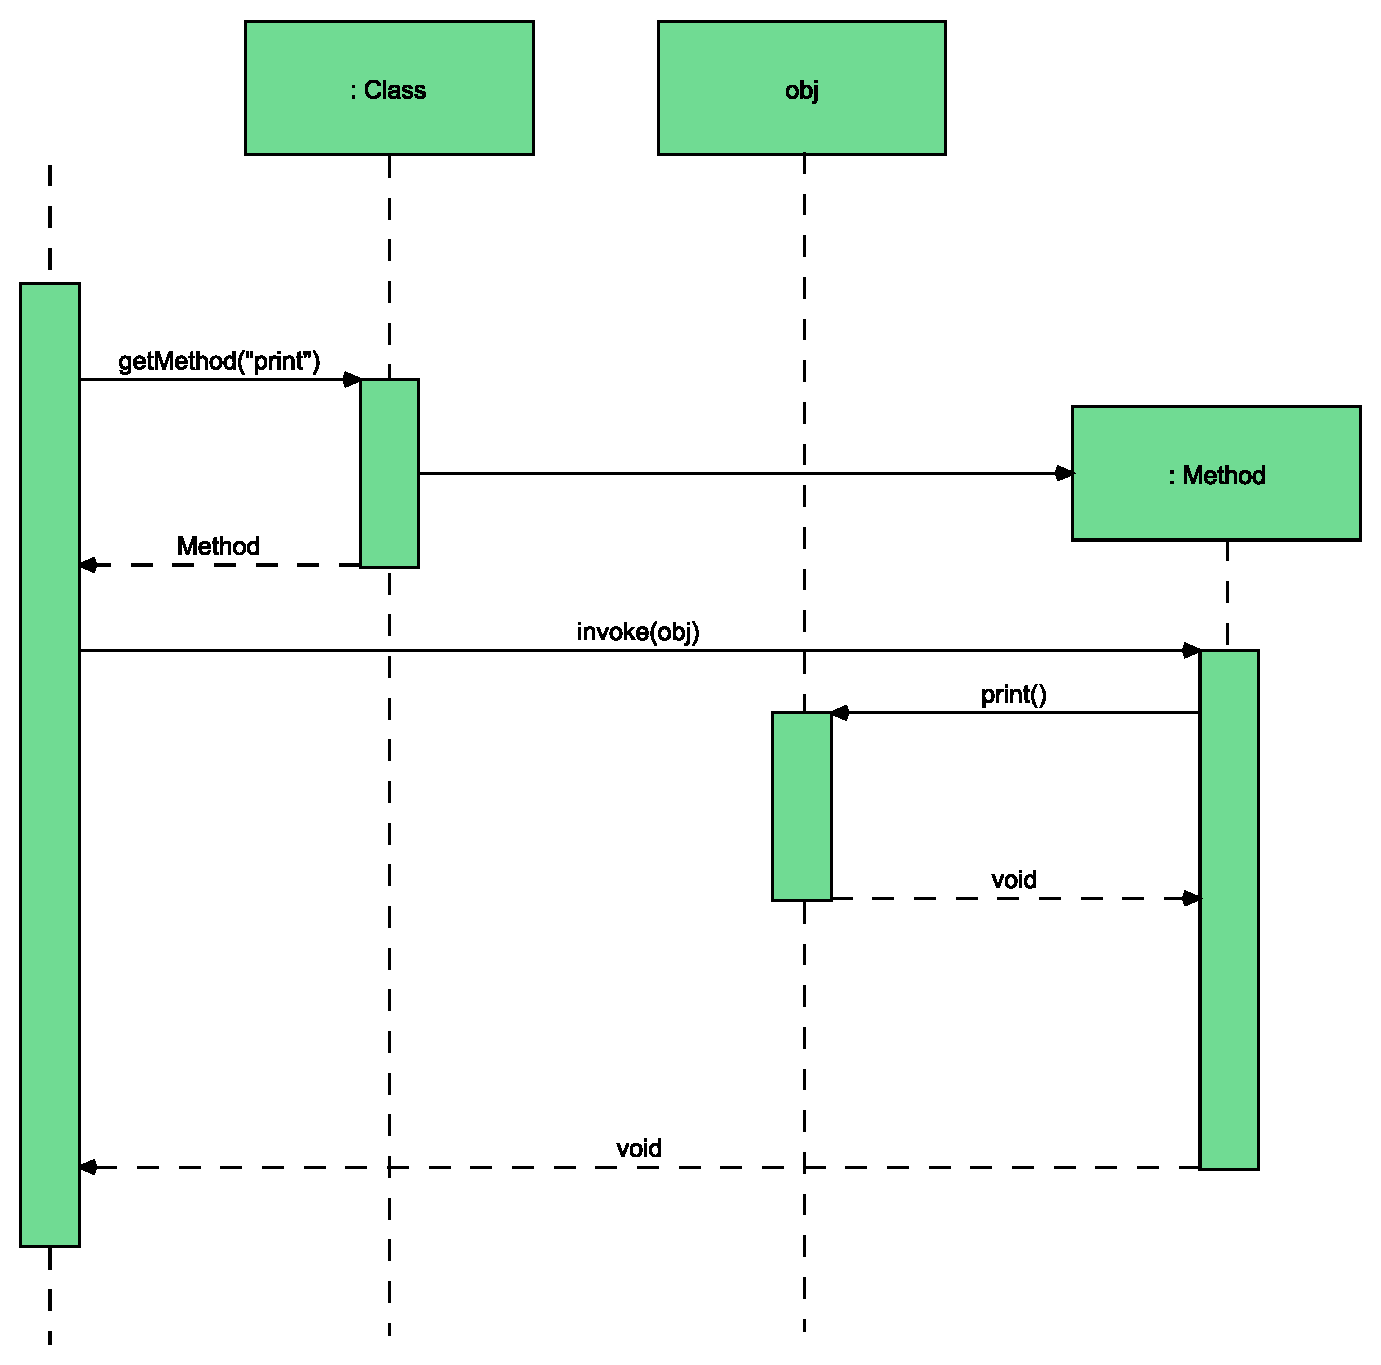
\includegraphics[width=0.8\textwidth]{material/images/flussReflection.pdf}
    \caption{Aufruf einer Methode \cite{Forman04javareflection}}
    \label{fig:refl-fluss}
  \end{figure}

  % Sequenzdiagram 
  In der Abbildung \ref{fig:refl-fluss} wird ein Ablauf eines Methodenaufrufs mithilfe von Reflection visualisiert. Im ersten Schritt muss die Methode gefunden werden. Da wir den Typen nicht kennen und nur für den Stammobjekt Typen deklarieren Methoden nutzen können, lassen wir das Objekt sich selbst inspizieren und die geforderte Methode finden. Dafür wird nach einer bestimmten Methode der Klasse gesucht und bei Erfolg ein Objekt von Typ \textit{Method} zurückgegeben. Das Methodenobjekt enthält die ganze Information über die gesuchte Methode, wie zum Beispiel Parameter und Rückgabewerte. Ausgerüstet mit der benötigten Information kann die Methode ausgeführt werden. Dafür braucht das Methodenobjekt eine Instanz der passenden Klasse sowie für die Ausführung benötigten Parameter. Nach der Abwickelung wird das Ergebnis der Ausführung vom der Objektinstanz über das Methodenobjekt zurück in den Programmfluss delegiert. \cite{Forman04javareflection} 

 % Nutzen: Felder Methode, Konstruktoren
  \bigbreak Somit sind die drei Hauptmerkmale einer Klasse ihre Felder, Methoden sowie Konstruktoren durch eine entsprechendes Java Objekt aus der Reflection-API repräsentiert. 

  \begin{itemize}
    \item java.lang.reflect.Field
    \item java.lang.reflect.Method
    \item java.lang.reflect.Constructor
  \end{itemize}

  Mithilfe des Klassen Typs können die oben genannten Objekte erzeugt und manipuliert werden. Diese bieten Schnittstellen für das Abfragen der Klassenstruktur an und repräsentieren Charakteristika der entsprechenden Klassen.

  \begin{itemize}
    \item Field[ ] *.class.getFields();
    \item Method[ ] *.class.getDeclaredMethods();
    \item Constructor[ ] *.class.getConstructors();
  \end{itemize}
  \bigbreak 

  Um den Zusammenhang und den Nutzen von Reflection darzustellen, wird in der Abbildung \ref{my-refl} ein Szenario durchgespielt, das eine unbekannten Typen mithilfe des Konstruktors initialisiert, dessen Methoden aufruft, das Feld bearbeitet und wiedergibt, ohne die Objektstruktur im Voraus zu kennen. Des Weiteren ist zu beachten, dass statische Klassenmethoden sowie private Felder und Methoden mithilfe von Reflection offen zugänglich gemacht werden können.\cite{Forman04javareflection}\bigbreak 

  % Bild mit Code der eine Objekt erstellt und Methoden aufruft. Mit Kommentaren zwischen den Zeilen.
  \begin{lstlisting}[caption=Reflection in Aktion,label=my-refl,captionpos=b]
    public static void getMethods(@NotNull Class clazz) throws
            NoSuchMethodException, NoSuchFieldException,
           InvocationTargetException, InstantiationException,
           IllegalAccessException {
      Method method;

        // Instantiierung
        Constructor[] ctors = clazz.getDeclaredConstructors();
        Object dynamic = ctors[0].newInstance(4);
        // Aufruf einer privaten Methode
        method = clazz.getDeclaredMethod("print", String.class);
        method.setAccessible(true);
        method.invoke(dynamic,"Hello World");
        // Feld Manipulation
        Field field = clazz.getDeclaredField("version");
        field.set(dynamic, 5);
        int version = (int) field.get(dynamic);
        System.out.println(version);
    }
  \end{lstlisting}

 % Wo wird Reflection genutzt, wieso ist es so nützlich in der Modernen Software-Entwicklung 
  Wie in der Abbildung \ref{my-refl} dargestellt ist Reflection ein mächtiges Werkzeug, das aus der morden Softwareentwicklung nicht wegzudenken ist und wird in zahlreichen Framework's verwendet, um den Entwickler zu unterstützen. 

  \begin{itemize}
    \item Zum Beispiel wird \textit{Dependency Injection} mithilfe von Reflection realisiert, indem ein Framework, wie zum Beispiel Spring, die entsprechende Implementierung für ein Interface sucht und initiiert. In Diesem Zusammenhang wird Anhand des \textit{implement} Schlüssels und zusätzlicher Meta-Information aus der Klassen \textit{Annotation} ein eindeutiger Kandidat auserwählt und konstruiert.
    \item Beim Serialisieren und Deserialisieren von Objekten werden die Objektfelder in JSON und wieder zurück konvertiert, ohne die Feldnamen sowie ihre Anzahl zu kennen.
    \item Die Web-Container Tomcat oder WildFly leiteten die Web-Anfragen an das entsprechende Modul durch das Analysieren der \textit{web.xml} und Anfordern der passenden URI.
    \item JUnit verwendet Reflection, um die Methoden einer Klasse nach Test-Annotation zu durchsuchen, um diesen anschließend aufzurufen.
  \end{itemize}

\section{Gradle}
Gradle ist ein Build-Tool ähnlich wie Maven und Ant. Gradle ist das neueste dieser drei Build-Tools, und wird zunehmend eingesetzt. Es ist Open Source und hat viel Akzeptanz bei den Entwicklern gefunden, da es auf die Erfahrung aus den vorhandenen genannten Build-Tools zurückgreift. Mehrere bekannte Projekte wie Android, Spring Framework und Hibernate haben ihre Build-Systeme bereits auf Gradle migriert. Einige der Vorteile, die Gradle gegenüber Maven und Ant hat, sind präzisere Erstellungsskripte und eine flexiblere Erstellungssprache.\bigbreak

\subsubsection{Beweggründe für Gradle}
Für die Migration von Ant auf Gradle werden im Folgenden die Schwächen von Ant gegenüber Gradle aufgelistet.
\begin{itemize}
  \item Die Verwendung von XML als Definitionssprache für die Erstellungslogik führt zu übermäßig großen und ausführlichen Erstellungsskripten im Vergleich zu Erstellungswerkzeugen mit einer prägnanteren Definitionssprache. \cite{muschko2014gradle}
  \item Komplexe Erstellungslogik führt zu langen und nicht verwaltbaren Erstellungsskripten. Der Versuch, bedingte Logik wie \textit{if-then}, \textit{for-each} oder \textit{while} Anweisungen mit XML zu definieren, wirkt unnatürlich und aufgeblasen.\cite{muschko2014gradle}
  \item Ant gibt keine Richtlinien zum Einrichten des Projekts. In einem Unternehmen führt dies häufig zu einer Build-Datei, die jedes Mal anders aussieht.\cite{berglund2011building}
  \item Gemeinsame Funktionen werden häufig kopiert und eingefügt. Jeder neue Entwickler im Projekt muss die individuelle Struktur eines Builds verstehen.\cite{varanasi2015introducing}
  \item Die Verwendung von Ant ohne Ivy erschwert das Verwalten von Abhängigkeiten. In vielen Fällen müssen die JAR-Dateien in die Versionskontrolle eincheckt und deren Organisation manuell verwaltet werden.\cite{varanasi2015introducing}
\end{itemize}

\subsubsection{Aufbau}
  Die gradle Umgebung besteht aus mehreren Komponenten. Jede von den Komponenten wird in einem bestimmten Lebenszyklus von Gradle für das Erstellen der Applikation genutzt.\newline
  Um Gradle zu starten, werden zwei Ausführbare Skripte mitgeliefert. Für die Ausführung auf dem \textit{Unix} basierte Systeme kann \textit{graldew} verwendet werden und für die Windows Ausführung ist das \textit{gralde.bat} Skript zuständig.\bigbreak
  \begin{figure}[h!]
    \centering
    \begin{minipage}{7cm}
      \dirtree{%
       .1 .
       .1 build.gradle.
       .1 gradle.
       .2 wrapper.
       .3 gradle-wrapper.jar.
       .3 gradle-wrapper.properties.
       .1 gradlew.
       .1 gradlew.bat.
       .1 settings.gradle.
       }
    \end{minipage}
    \caption{Gradle Konfiguration}
    \label{fig:gradle_project}
  \end{figure}

  Nach dem Anstoßen des Ausführung Skripts, wird Gradle konfiguriert und setzt eine bestimmte Zielversion für die Ausführung fest. Dies geschieht innerhalb der \textit{gradle/wrapper} Ordnerstruktur und initiiert Gradle für die Ausführung. Als nächstes sammelt Gradle die Information über alle Teilnehmer der Projektorganisation und legt eine globale Projektstruktur für die Ausführung fest. Dafür wird in der Initialisierungsphase die \textit{settings.gradle} der Projekte und die Lokale \textit{init.gradle} Konfigurationsdatei ausgelesen. Diese bestimmen Umgebungsvariablen, Eigenschaften und persönlichen Informationen. Des Weiteren werden teilnehmende Projekte gesetzt und instantiiert.\newline
  Nachdem die Initialisierungsphase beendet ist, werden erstellte Projekte konfiguriert. Die Konfiguration geschieht laut den \textit{build.gradle} Konfigurationsdatei und bereitet die Projekte für die Ausführung vor. Zum Schluss wird das Bauen durchgeführt, indem eine Reihe von Ausführungsschritten (Tasks) von dem Nutzer aufgerufen werden.\cite{mitra2015mastering}


\subsubsection{Gradle build Skript}
\begin{lstlisting}[caption=Gradle in Aktion \cite{ikkink2015gradle},label=my-grl,captionpos=b]

  // Deklaration der genutzten Plugins 
  plugins {
      id 'java'
  }
  // Bibliothek Quellen 
  repositories {
      mavenCentral()
  }
  // Projektabhángigkeiten
  dependencies {
      compile('javax:javaee-web-api:8.0')
  }
  // Klassenpfade 
  configurations {
    libs
    plugins
    compile
  }
  // Felder
  group 'de.firm'
  description 'my first application'
  version version
  defaultTasks 'war'
  // Projektstruktur
  sourceSets {
      main {
          java {
              srcDirs ['src/main/java']
              webAppDirName 'src/main/webapp'
              outputDir file('out/classes')
          }
          resources {
              srcDirs ['src/main/resources']
              output.resourcesDir = file('out/resources')
          }
      }
  }
  // Konfiguration eines Abarbeitungsschritts
  task war {
      setGroup("gradle")
      setArchivesBaseName(name)
      webInf {
          into('classes') {
              from sourceSets.main.java.outputDir
              into('META-INF') {
                  from(sourceSets.main.resources.files) {
                      include("persistence.xml")
                  }

              }
          }
      }
      metaInf {
          from(sourceSets.main.resources) {
              include("import.sql")
          }
          manifest {
              attributes 'version': war_version
              attributes 'description': war_description
              attributes 'creator': war_creator
              attributes 'classifire': war_classifire
          }
      }
  }
  // Task Graph Manipulation 
  deploy.dependsOn(war)
\end{lstlisting}

In der Abbildung \ref{my-grl} ist eine Standard Struktur eines Gradle Build Skript abgebildet, die mit einem Java Plugin arbeitet und ein war Archiv erstellt. 


% \subsubsection{OSGi}


% \subsubsection{Docker}
% \subsubsection{JavaScript}
% \subsubsection{TypeScript}
% \subsection{Java Umsetzung} 
% % wie es war mit 1.8
% % was draus gewirden ist in 9
% \newpage

% \section{Vergleich mit anderen Modularisierungskonzepten}


% \subsection{Jigsaw}
% % wie löst java 9 die Probleme 
% % theoretisch 
% \subsection{Modular JDK}
% % bevor entwickler modularisieren muss da System selbst modular sein.
% % eine beispiel umsetzung
% % löst probleme von beginn an, praktische umsetzung 
% \subsection{Modulstruktur}
% % arten von modulen 
% % inhalt und aufbau
% % zugriffsberechtigungen 
% \subsection{Modulepfad}
% % classloader änderungen 
% % verweist nicht mehr auf klassen orte sondern auf  modul Orte
% \subsection{Optionale Abhängigkeiten}
% %  optionale erweiterbarkeit
% \subsection{Reflection}
% %  sicherer und braucht explizite konfiguration 
% % zugriff auf  alle klassen nicht mehr möglich 
% \subsection{Services} 
% \subsection{Migration}

% \section{Vergleich mit anderen Modularisierungskonzepten}


% \section{Modularisierungskonzepten}

% \subsection{Java Plattform Module System}

% \subsection{Vergleich mit anderen Modularisierungskonzepten}

% \subsection{Vom Classpath zum Modulpath}

% \subsection{Arten von Jigsaw-Modulen}

% \subsection{Service-Provider und -Consumer}

% \subsection{Abhängigkeitsgraph mit Graphviz}


% - Module gabs schon lagne 
% - osg 
% - und und und 
% - angular 